\documentclass[border=6pt]{standalone}
\usepackage{tikz}
\usetikzlibrary{arrows.meta}
\begin{document}
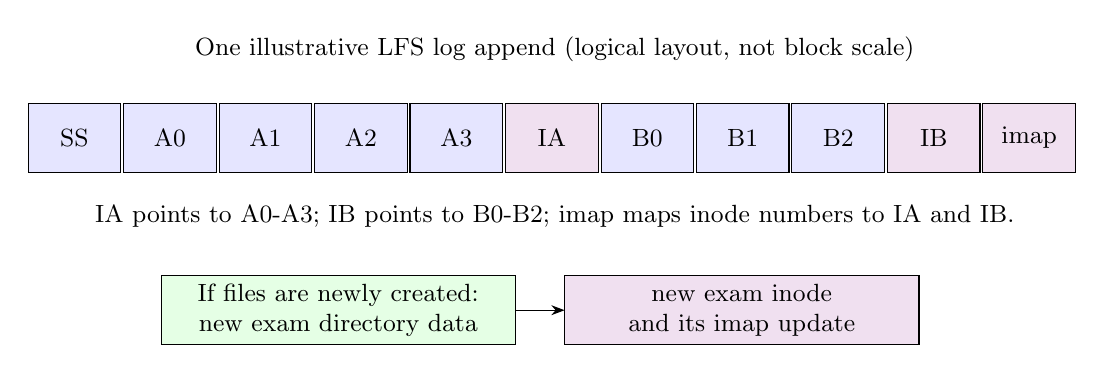
\begin{tikzpicture}[>=Stealth]
\node[align=center,font=\small] at (6.875,4.375) {One illustrative LFS log append (logical layout, not block scale)};
\draw[fill=blue!10] (0.188,3.688) rectangle (1.363,2.812);
\node[align=center,font=\small] at (0.775,3.250) {SS};
\draw[fill=blue!10] (1.400,3.688) rectangle (2.575,2.812);
\node[align=center,font=\small] at (1.988,3.250) {A0};
\draw[fill=blue!10] (2.612,3.688) rectangle (3.788,2.812);
\node[align=center,font=\small] at (3.200,3.250) {A1};
\draw[fill=blue!10] (3.825,3.688) rectangle (5.000,2.812);
\node[align=center,font=\small] at (4.412,3.250) {A2};
\draw[fill=blue!10] (5.037,3.688) rectangle (6.213,2.812);
\node[align=center,font=\small] at (5.625,3.250) {A3};
\draw[fill=violet!12] (6.250,3.688) rectangle (7.425,2.812);
\node[align=center,font=\small] at (6.838,3.250) {IA};
\draw[fill=blue!10] (7.463,3.688) rectangle (8.637,2.812);
\node[align=center,font=\small] at (8.050,3.250) {B0};
\draw[fill=blue!10] (8.675,3.688) rectangle (9.850,2.812);
\node[align=center,font=\small] at (9.262,3.250) {B1};
\draw[fill=blue!10] (9.887,3.688) rectangle (11.062,2.812);
\node[align=center,font=\small] at (10.475,3.250) {B2};
\draw[fill=violet!12] (11.100,3.688) rectangle (12.275,2.812);
\node[align=center,font=\small] at (11.688,3.250) {IB};
\draw[fill=violet!12] (12.312,3.688) rectangle (13.488,2.812);
\node[align=center,font=\small] at (12.900,3.250) {imap};
\node[align=center,font=\small] at (6.875,2.250) {IA points to A0-A3; IB points to B0-B2; imap maps inode numbers to IA and IB.};
\draw[fill=green!10] (1.875,1.500) rectangle (6.375,0.625);
\node[align=center,font=\small] at (4.125,1.062) {If files are newly created:\\new exam directory data};
\draw[fill=violet!12] (7.000,1.500) rectangle (11.500,0.625);
\node[align=center,font=\small] at (9.250,1.062) {new exam inode\\and its imap update};
\draw[->] (6.375,1.062) -- (7.000,1.062);
\end{tikzpicture}
\end{document}
